% Template for Cogsci submission with R Markdown

% Stuff changed from original Markdown PLOS Template
\documentclass[10pt, letterpaper]{article}

\usepackage{cogsci}
\usepackage{pslatex}
\usepackage{float}
\usepackage{caption}

% amsmath package, useful for mathematical formulas
\usepackage{amsmath}

% amssymb package, useful for mathematical symbols
\usepackage{amssymb}

% hyperref package, useful for hyperlinks
\usepackage{hyperref}

% graphicx package, useful for including eps and pdf graphics
% include graphics with the command \includegraphics
\usepackage{graphicx}

% Sweave(-like)
\usepackage{fancyvrb}
\DefineVerbatimEnvironment{Sinput}{Verbatim}{fontshape=sl}
\DefineVerbatimEnvironment{Soutput}{Verbatim}{}
\DefineVerbatimEnvironment{Scode}{Verbatim}{fontshape=sl}
\newenvironment{Schunk}{}{}
\DefineVerbatimEnvironment{Code}{Verbatim}{}
\DefineVerbatimEnvironment{CodeInput}{Verbatim}{fontshape=sl}
\DefineVerbatimEnvironment{CodeOutput}{Verbatim}{}
\newenvironment{CodeChunk}{}{}

% cite package, to clean up citations in the main text. Do not remove.
\usepackage{apacite}

% KM added 1/4/18 to allow control of blind submission


\usepackage{color}

% Use doublespacing - comment out for single spacing
%\usepackage{setspace}
%\doublespacing


% % Text layout
% \topmargin 0.0cm
% \oddsidemargin 0.5cm
% \evensidemargin 0.5cm
% \textwidth 16cm
% \textheight 21cm

\title{Estimating demographic bias on tests of children's early vocabulary}


\author{{\large \bf George Kachergis (kachergis@stanford.edu)} \AND {\large \bf Nathan Francis (nathan99@stanford.edu)} \AND {\large \bf Michael C. Frank (mcfrank@stanford.edu)} \\ Department of Psychology, Stanford Unviersity \\ Stanford, CA 94305 USA }


\begin{document}

\maketitle

\begin{abstract}
Children's early language skill has been linked to later educational
outcomes, making it important to measure early language accurately.
Parent-reported instruments such as the Communicative Development
Inventories (CDIs) have been shown to provide reliable and valid
measures of children's aggregate early language skill. However, CDIs
contain hundreds of vocabulary items, some of which may not be heard
(and thus learned) equally often by children of varying backgrounds.
This study used a database of American English CDIs to identify words
demonstrating strong bias for particular demographic groups of children,
on dimensions of sex (male vs.~female), race (white vs.~non-white), and
maternal education (high vs.~low). For each dimension, we identified
dozens of strongly biased items, and showed that eliminating these items
reduced the expected ability difference between groups. Additionally, we
investigated how well the relative frequency of words spoken to young
girls vs.~boys predicted sex-based word learning bias, and discuss
possible sources of demographic differences in early word learning.

\textbf{Keywords:}
language acquisition; word learning; measuring instrument bias;
demographic bias
\end{abstract}

\hypertarget{introduction}{%
\section{Introduction}\label{introduction}}

Researchers, clinicians, and parents have long been fascinated with the
surprising speed and variability in the growth of young children's
vocabulary. Children's early vocabulary growth is assumed to reflect not
only their exposure to child-directed speech, but also the varying
difficulty of different types of words, and individual differences in
the aptitude of the child -- including potential language deficits.
Children show both consistency in some skills across development, as
well as significant influence from external factors. For example,
Bornstein, Hahn, \& Putnick (2016) found stability in core language
skills across 10 years of children's development, despite changes in
maternal income and education over the study period.

Yet there are consistent demographic predictors of early vocabulary.
Maternal education, often used as a proxy for socioeconomic status
(SES), is associated with children's language processing and vocabulary
by 18 months (Fernald, Marchman, \& Weisleder, 2013), and is predictive
of later educational outcomes (Marchman \& Fernald, 2008; see Schwab \&
Lew-Williams, 2016 for review). Other factors are also predictive of
language skill: first-born children tend to outpace their siblings, and
female children tend to have better language skills than their
age-matched male counterparts (Eriksson et al., 2012; Frank, Braginsky,
Yurovsky, \& Marchman, 2021) -- a sex-based verbal advantage that
continues through high school (see Petersen, 2018 for a review).

One challenge in comprehensive assessment of these differences is that
it is difficult to get a complete measure of young children's language
skill. Long recordings are prohibitively difficult to collect and
transcribe, and yet any short recording (e.g., a 1-hour play session)
will elicit only a small proportion of the words and constructions that
children know. Thus, researchers of early word learning have constructed
tests with hundreds of words, intentionally oversampling words that are
more likely to be known by young children.

We focus here on the MacArthur-Bates Communicative Development
Inventories (CDIs; Fenson et al., 1994, 2007), a set of parent-reported
measures of children's productive and receptive language skills, which
offer a low-cost and reliable way to estimate children's early language
skills (Fenson et al., 1994). CDIs have shown good predictive validity
(e.g., Fenson et al., 1994; Bornstein \& Putnick, 2012; Duff, Reen,
Plunkett, \& Nation, 2015). Our primary focus is the vocabulary
checklist portion of the CDI Words \& Sentences (CDI:WS) form, comprised
of 680 early-learned words across 22 categories (e.g., animals,
vehicles, action words, pronouns) selected to assess the productive
vocabulary of children 16 to 30 months of age. For each item on the
CDI:WS, caregivers are asked to respond whether the target child has
been heard to say (i.e.~produce) the given item. Children's total
vocabulary score on the CDI:WS is tightly correlated with other facets
of early language (e.g., grammatical competence and gesture), suggesting
that the language system is ``tightly woven'' (Frank et al., 2021). Due
to these desirable properties, CDIs have been adapted to dozens of
languages, and a central repository of CDI data contributed from all
over the world has been created (Wordbank; Frank, Braginsky, Yurovsky,
\& Marchman, 2017; Frank et al., 2021).

CDIs are a useful tool for measuring demographic effects because of
their wide use across languages. But their use in this context poses a
chicken and egg problem. While it is possible that there is an
underlying difference in mean language ability between demographic
groups, CDIs could also have bias for or against particular groups based
on the words they include.

The idea that some items on a test may show bias, favoring one group
over another, is known in psychometrics as Differential Item Function
(DIF; Holland \& Wainer (1993){]}. DIF can decrease the validity of a
test, as the test may be overestimating the ability of test-takers in
one group and underestimating the ability of another group -- not
because of any underlying mean difference in ability between the groups,
but simply because the test is unfair (Camilli, 2013). For example, if a
vocabulary test is composed almost entirely of the names of farm
equipment, the test will underestimate the knowledge of urban children,
who have experience of other contexts, despite being less familiar with
farm equipment than their rural peers. Of course, there may be an
ability difference between demographic groups, as is likely the case for
the female language advantage, which has been documented in many
languages (Eriksson et al., 2012; Frank et al., 2021). And both
observations could be true -- a test could be biased to inflate a true
demographic difference.

Our goal in the current study is to use DIF analyses to assess these
possibilities. Specifically, we test the 680 vocabulary items on the
American CDI:WS for DIF along three dichotomized demographic dimensions:
sex (male vs.~female), maternal education (no more than secondary vs.~at
least some college), and race (white vs.~non-white).

The outline of this paper is as follows. First, we introduce the
Wordbank data and the IRT model, and examine the overall size of
demographic differences in early word learning based on the full CDI:WS.
We then fit the IRT model to both groups for each demographic factor,
and look at the item parameters for evidence of DIF, noting in
particular how many items are significantly biased in favor of each
group, and describing them qualitatively. Next, we use these item
parameters to systematically prune biased items from the CDI:WS, and
examine how the estimated size of demographic differences change as we
prune more items. Finally, using a corpus of child-directed speech, we
examine the extent to which variation in word frequencies heard by boys
vs.~girls predicts sex-based DIF. Based on these analyses, we provide
recommendations for next steps to be taken to identify and potentially
replace items on the CDI showing demographic bias.

\hypertarget{methods}{%
\section{Methods}\label{methods}}

\hypertarget{vocabulary-data}{%
\subsection{Vocabulary Data}\label{vocabulary-data}}

\hypertarget{participants}{%
\subsubsection{Participants}\label{participants}}

We analyzed parent-reported Wordbank data from 5520 American English
CDI: Words \& Sentences administrations for children 16 to 30 months of
age (Frank et al., 2017, 2021). Full demographic data are not reported
in some datasets contributed to Wordbank: sex was available for 4094
children, race/ethnicity was available for 2715 children, and maternal
education (a proxy for socioeconomic status; SES) was available for 5520
children.

The analysis of sex-based differences included CDI administrations from
1989 female and 2105 male children. The analysis of race-based
differences included data from 2202 white, 67 Asian, 222 Black, 131
Hispanic, and 93 ``Other'' children. Due to sparse data for many
categories, we binarized participants' race and ethnicity as White
(2202) or Non-white (513), recognizing that there is important variation
between groups that this will fail to capture. Data for the maternal
education analysis included CDI data from children whose mothers had the
following levels of education: 8 with no more than primary school
education, 123 with some secondary school, 416 with no more than
secondary school, 613 with some college, 870 with no more than a college
degree, 162 with no more than some graduate school, and 584 with a
graduate degree. Again due to data sparsity, we binarized the 4973
children whose mothers had at least some college or more as high
maternal education (high-ME), and those whose mothers had at most high
school (547 children) as low maternal education (low-ME).

\hypertarget{rasch-model}{%
\subsection{Rasch Model}\label{rasch-model}}

The Rasch model, also known as the 1-parameter logistic (1PL) model, is
the simplest Item Response Theory model, and is thus the easiest to use
to investigate potential differences in item function across different
groups of participants. The Rasch model jointly estimates for each child
\(j\) a latent ability \(\theta_j\), and for each item \(i\) a
difficulty parameter \(b_i\). In the model, the probability of child
\(j\) knowing (i.e., producing or understanding) a given item \(i\) is

\[P_{i}(x_i = 1 | b_{i},\theta_j ) = \frac{1}{1 + e^{-D(\theta_j - b_i )}}\]

\noindent where \(D\) is a constant scaling parameter (\(D=1.702\))
which makes the logistic closely match the ogive function in traditional
factor analysis (Chalmers, 2012; Reckase, 2009). Child ability
(\(\theta\)) and item difficulty (\(b\)) distributions are standardized
(i.e., mean of 0), and expected to be normally-distributed. Children
with high latent ability (\(\theta\)) will be more likely to produce any
given item than children with lower latent ability, and more difficult
items will be produced by fewer children (at any given \(\theta\)) than
easier items.

In the multigroup Rasch model, an item's difficulty is allowed to vary
by group. For example, in the sex-based multigroup model, item \(i\)'s
difficulty is \(b_{i}^{female}\) for females, and \(b_{i}^{male}\) for
males. To identify DIF, a multigroup Rasch model will be fitted for each
demographic dimension of interest (sex, maternal education, and
ethnicity), and we will examine the between-group difficulty difference
for each item (e.g., \(d_i = b_{i}^{female} - b_{i}^{male}\)). If there
is no DIF for a given item, then \(d_i \approx 0\) as the two groups
find the item equally difficult.

\hypertarget{results}{%
\section{Results}\label{results}}

First, we examine the size of demographic effects on language ability in
a baseline Rasch model fitted without regard to demographic group. Then
we fit a multigroup Rasch model for each demographic factor, and
characterize the between-group differences in item difficulties. Next,
we re-examine the size of demographic effects after pruning biased items
from the CDI:WS using different criteria, and recommend a threshold.
Finally, we measure the strength of association between sex-related
differences in language input and the degree of sex-related DIF. The
scripts and models needed to reproduce our analyses are available on
\href{https://osf.io/57rsw/?view_only=2b6ecb61fe08458293af7421d276932a}{OSF}.

\begin{CodeChunk}
\begin{figure*}[t]

{\centering \includegraphics[width=\linewidth]{figs/baseline-ability-vs-age-hor-1} 

}

\caption[Language ability vs]{Language ability vs. age by demographic group, from the baseline Rasch model.}\label{fig:baseline-ability-vs-age-hor}
\end{figure*}
\end{CodeChunk}

\hypertarget{demographic-effects-in-the-baseline-rasch-model}{%
\subsection{Demographic effects in the baseline Rasch
model}\label{demographic-effects-in-the-baseline-rasch-model}}

We fit a baseline Rasch model to the entire dataset, without demographic
information. Figure 1 shows children's language ability vs.~age by
demographic group from the baseline Rasch model, which assumes no DIF
(i.e., equal item parameters for all groups). A linear regression for
each demographic group, with age (centered) and its interaction, showed
significant effects. Female children had higher language ability than
male children (\(\beta=0.56\), \(p<.001\)), with no significant
interaction with age (\(\beta=0.02\), \(p=.10\)). High-SES children had
higher language ability than low-SES children (\(\beta=0.23\),
\(p=.02\)), an advantage that grew with age (\(\beta=0.11\),
\(p<.001\)). White children had higher language ability than non-white
children (\(\beta=0.50\), \(p<.001\)), an advantage that grew with age
(\(\beta=0.08\), \(p<.001\)). We will re-examine these demographic
regressions after trimming items showing extreme DIF.

\hypertarget{identifying-biased-cdi-items}{%
\subsection{Identifying biased CDI
items}\label{identifying-biased-cdi-items}}

To aid in identifying CDI items with DIF we created GLIMMERs (Graphs of
Logits Imputed Multiply with Means Equal; Stenhaug, Frank, \& Domingue
(2021)), which visualize between-item variation in group performance
differences. These parameters are drawn from a fitted multigroup Rasch
model for each demographic variable (sex, SES, and race), with the
assumption that the mean language ability in each group is the same
(e.g.~for sex, \(\mu_{male}=\mu_{female}=0\)), thus pushing all
between-group variation into the item difficulty parameters. For the
case of sex, where we believe \(\mu_{female}>\mu_{male}\), this means we
may expect to find many items with difficulty
\(b_i^{female} < b_i^{male}\), but we can still examine the distribution
of differences in item difficulty (\(d_j = b_i^{male} - b_i^{female}\))
for outliers. GLIMMER plots show distributions of parameter differences
rather than point estimates to convey the uncertainty about the
existence of DIF. These distributions are generated by drawing 10,000
imputations from the item parameter covariance matrix.

Figure 2 shows GLIMMERs for a selection of CDI items for sex (left),
maternal education (middle), and race (right). The full GLIMMERs, with
all 680 CDI:WS items, are available on
\href{https://osf.io/57rsw/?view_only=2b6ecb61fe08458293af7421d276932a}{OSF},
but were too large to include here. It is important, however, to inspect
the full plots, for if there is a cluster of items in a GLIMMER, the
analyst may conclude that these items are strong candidates for DIF on
that dimension. For example, there is some clustering at the top and
bottom of the sex GLIMMER (Fig. 2, left): at the top,
``vagina''\footnote{Parents using the CDI are instructed to check
  genital items if the child produces whatever word the family uses.},
``tights'', ``dress (object)'', and ``doll'' form a cluster of items
that are much more well-known for females, while at the bottom,
``penis'' stands out as much more well-known by males. For the maternal
education and race GLIMMERs -- and in the rest of the full sex GLIMMER,
there are not clusters, but rather a continuum of smoothly varying
differences with overlap. This pattern makes identifying items with DIF
quite difficult, as different methods are likely to yield inconsistent
results (Stenhaug et al., 2021). Hence, we next characterized the
distributions of the item-level group difficulty differences, and
measured the influence of pruning a varying number of items on the
demographic effect sizes.

\begin{CodeChunk}
\begin{figure*}[h]

{\centering 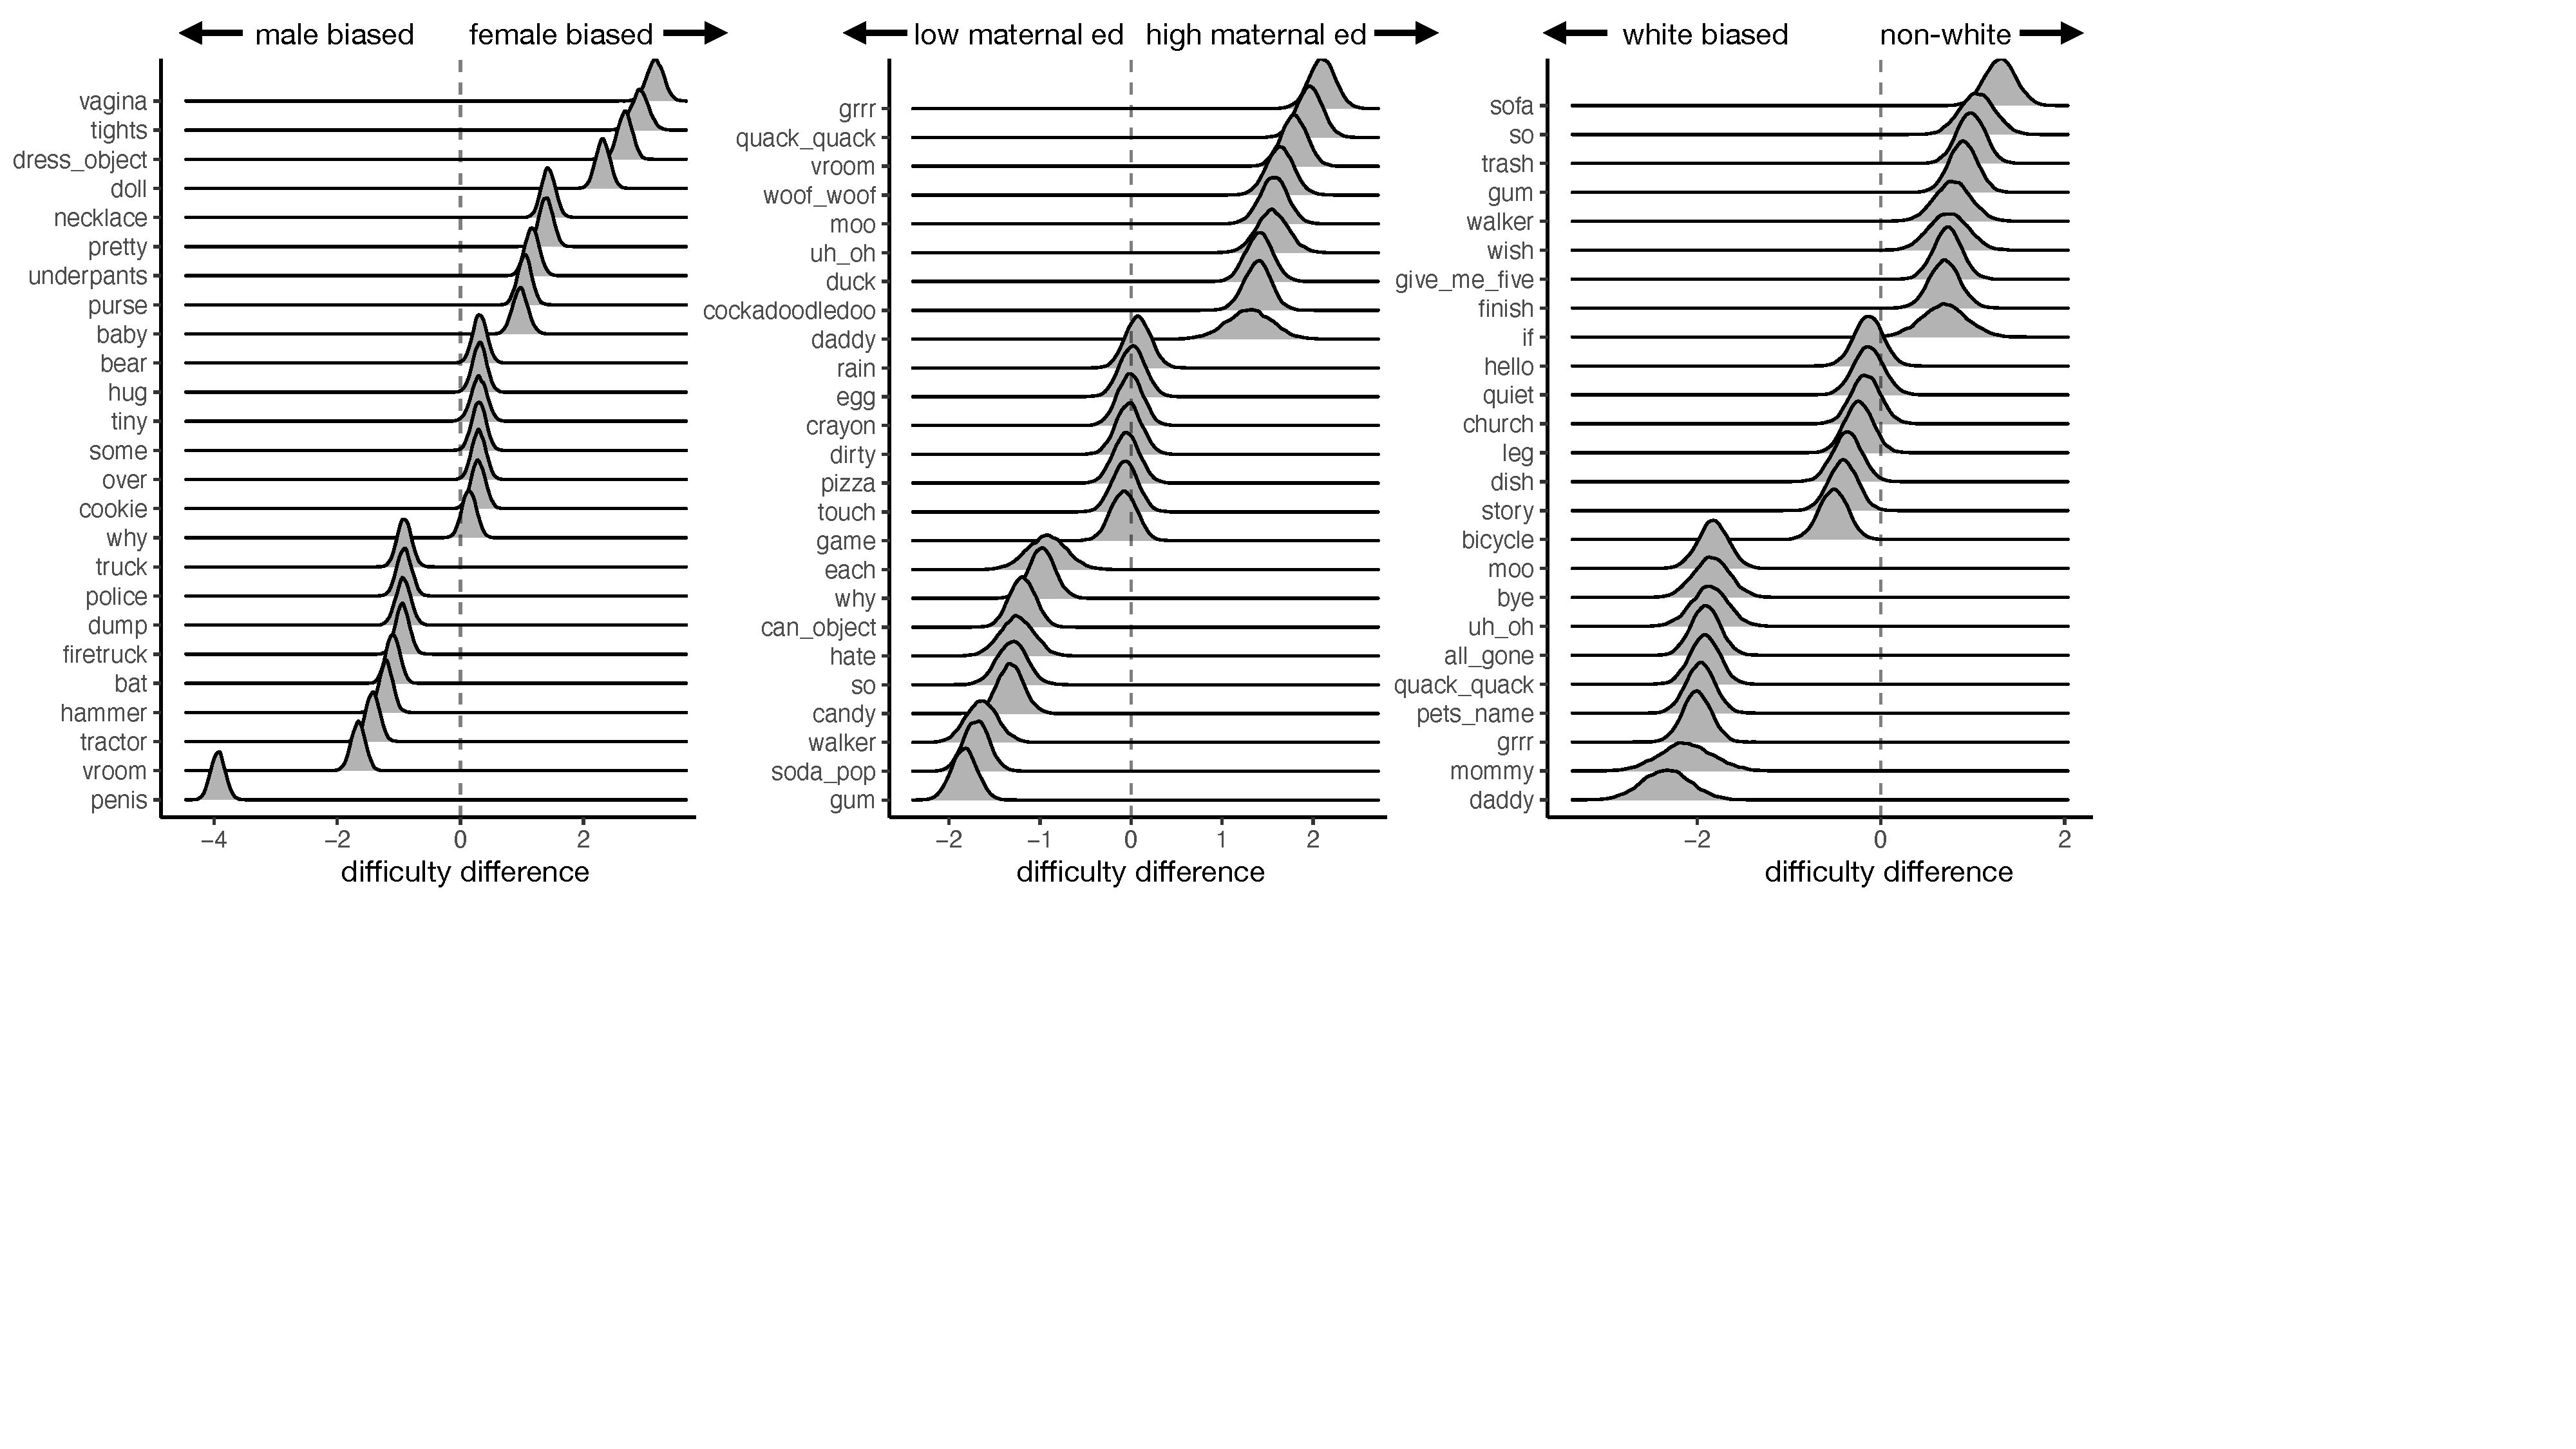
\includegraphics[width=\linewidth]{figs/smGLIMMER_combo} 

}

\caption[GLIMMER plots of a sample of CDI:WS words from the sex bias model (left), the maternal education model (center), and the race model (right)]{GLIMMER plots of a sample of CDI:WS words from the sex bias model (left), the maternal education model (center), and the race model (right). Words at the top are more well-known by one group (e.g., females, for sex), while those at the bottom are more known by the other group (e.g., males), and the selection in the middle show roughly the median difficulty difference for those groups.}\label{fig:glimmer-combo}
\end{figure*}
\end{CodeChunk}

\begin{CodeChunk}
\begin{figure*}[h]

{\centering \includegraphics[width=\linewidth]{figs/pruned-coefs-hor-1} 

}

\caption[Size of demographic effects (regression coefficients) with different pruning thresholds]{Size of demographic effects (regression coefficients) with different pruning thresholds.}\label{fig:pruned-coefs-hor}
\end{figure*}
\end{CodeChunk}

\hypertarget{sex}{%
\subsubsection{Sex}\label{sex}}

For sex, the median difficulty difference (male-female) was 0.28
(M=0.27, sd=0.4), with 593/680 items being easier for females than
males. The fact that the bulk of this distribution favors females shows
that the female language advantage is pervasive across the CDI:WS, and
suggests that it is likely to reflect more than the effect of a small
number of biased words (cf.~Frank et al., 2021).

\hypertarget{maternal-education}{%
\subsubsection{Maternal Education}\label{maternal-education}}

For maternal education (ME), the median difficulty difference (low-high)
was -0.01 (M=0.03, sd=0.55), with 337/680 items being easier for high-ME
than low-ME children. With the mean and median difficulty differences
close to 0, and roughly half of the words favoring each ME group, it
seems that the CDI:WS items are somewhat balanced with respect to ME
(and thus SES, by proxy).

\hypertarget{race}{%
\subsubsection{Race}\label{race}}

For race, the median difficulty difference (nonwhite-white) was 0.4
(M=0.46, sd=0.55), with 549/680 items being easier for white than
non-white children, revealing a fairly pervasive advantage for white
children on CDI items.

\hypertarget{demographic-effects-after-pruning}{%
\subsection{Demographic effects after
pruning}\label{demographic-effects-after-pruning}}

If only a small number of items show DIF, pruning decisions are simple;
this situation was not the case for any of the three characteristics we
examined. Instead, distributions of DIF varied smoothly by each
demographic factor. Thus, we chose to evaluate multiple thresholds for
pruning the extreme-valued items from each distribution. For each
demographic factor, we pruned items with a between-group difficulty
difference from the mean difference at varying thresholds, from
\textgreater.25 SD to \textgreater3 SD, in increments of .25 SD. At each
SD threshold, a potentially different subset of items are excluded for
each model, but with the goal of creating a single CDI that is less
biased on all dimensions, we pruned the union of the subsets excluded
from each model. For example, pruning \textgreater2SD from the mean of
each model excluded 25 sex-biased items, 39 ME-biased items, and 31
race-biased items, with their union being 76 unique items. Figure 3
shows the demographic effects (\(\beta\)s) at different exclusion
thresholds.

Ideally, we would find a single threshold that minimized the magnitude
of coefficients (and thus bias) for all three demographics
simultaneously. Unfortunately, the effect size for each demographic
variable was smallest (closest to 0) at different exclusion thresholds.
The effect size of sex was smallest when almost all items were trimmed
(\textgreater0.25 SD; \(\beta_{sex} = -.47\); 661/680 total items
trimmed; 433 due to sex extremity). The effect size of maternal
education (SES) was smallest when items \textgreater1.25SD in difficulty
difference were trimmed (\(\beta_{ME} = -.17\); 234 total items trimmed;
126 due to ME extremity). The effect size of race was minimized when
items more extreme than 0.5 SD were trimmed (\(\beta_{race} = .42\); 577
total items trimmed; 425 due to race extremity).

Where is the exclusion threshold that jointly minimizes the effect sizes
of these demographic variables? The strict exclusion of all items with
\textgreater.25 SD difficulty difference -- 661/680 (97\%) of the CDI:WS
-- best optimized this, but seems far too extreme of a culling. The next
best thresholds are \textgreater.5 SD -- again, too extreme -- or 3 SD,
a remarkably lax criterion that only excludes 19 items in total (11 due
to sex bias). Only slightly worse than these is \textgreater2.25 SD,
which excludes 59 items (9\%), and shows a modest effect of both race
(\(\beta=0.48\)) and maternal education (\(\beta=.19\)), and a
near-median effect size for sex (\(\beta=-.59\)). We characterize these
59 potentially biased items below, and consider whether we might
recommend pruning them from the CDI:WS.

\hypertarget{characterizing-biased-items}{%
\subsection{Characterizing biased
items}\label{characterizing-biased-items}}

Figure 4 shows the 59 items showing extreme bias (i.e., whose difficulty
was \textgreater2.25 SD from the mean difficulty difference on one or
more demographic dimension). There were 22 items with extreme sex-based
difficulty differences, only 7 of which were more known by females, with
the other 15 items favoring males. All but one of the sex-biased items
are nouns, many of which are stereotypically associated with one gender
more than the other, including stereotypically-male professions (e.g.,
``fireman''). For maternal education, 27 extrema were identified, only
10 of which were biased for low-SES children. As for sex, most of the
ME-biased items are nouns (15/27). Notably, many of the items more known
by high-ME children were animals (``zebra'', ``owl'') and animal sounds
(``baa baa'', ``moo''). Items more known by low-ME children include a
few sweet treats: ``candy'', ``soda/pop'', and ``gum''. For race, 21
extrema were identified, only 8 of which were easier for non-white
children. The lexical class of the race-biased items was more varied: 10
were nouns, but many others were early-learned words and phrases (e.g.,
``up'', ``all gone'', ``uh-oh'', ``bye'', ``mommy''). Only 10 of the 59
items were extreme in more than one model, with most of the overlap
being between race and ME (8 items). Only 1 item (``vroom'') was extreme
for all three demographics.

\begin{CodeChunk}
\begin{figure}[h]

{\centering 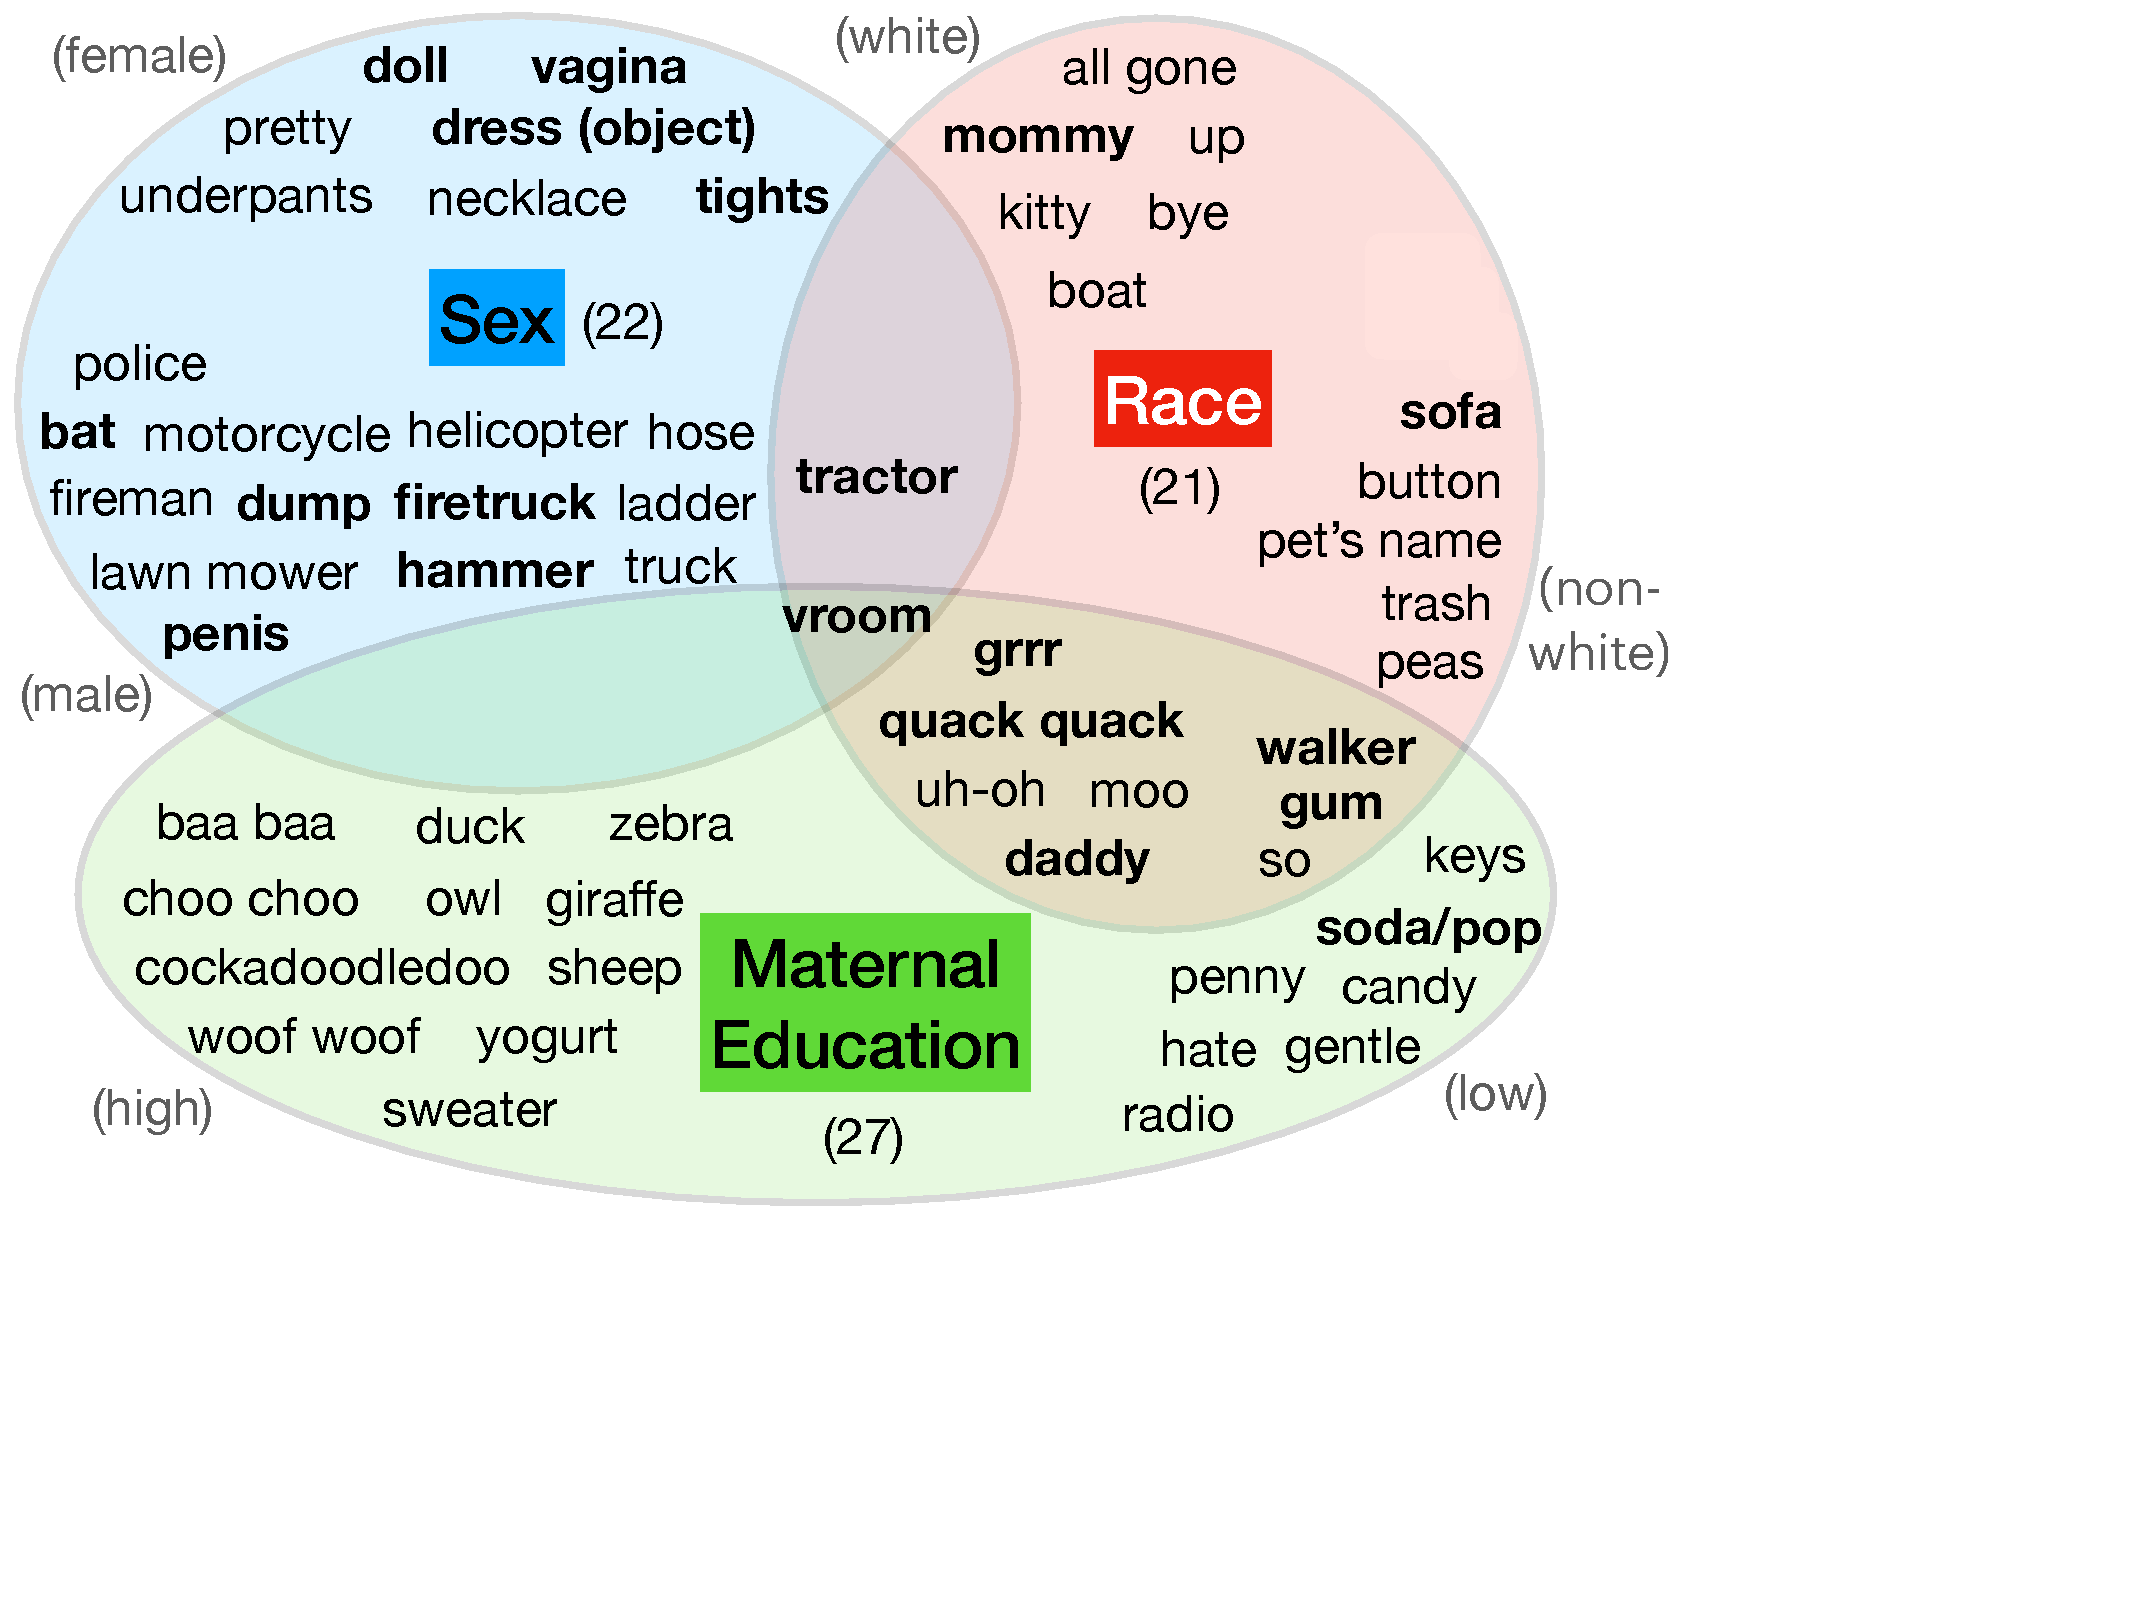
\includegraphics[width=\linewidth]{figs/extrema2p25sd_3sd_bold} 

}

\caption[The 59 items showing extreme bias (difficulty difference $>2.25$ SD) for one or more demographic]{The 59 items showing extreme bias (difficulty difference $>2.25$ SD) for one or more demographic. The 19 items in bold are those showing a difference $>3$ SD.}\label{fig:biased-words}
\end{figure}
\end{CodeChunk}

\hypertarget{relating-child-directed-speech-to-demographic-bias}{%
\subsection{Relating child-directed speech to demographic
bias}\label{relating-child-directed-speech-to-demographic-bias}}

Demographic differences in language ability are likely to be at least
partially explained by differences in linguistic input received by
children in different groups. Indeed, input quantity (total daily
tokens) and some measures of quality (e.g., lexical diversity: ratio of
word types vs.~tokens) have often been predictive of language learning
outcomes in demographic studies (Huttenlocher, Haight, Bryk, Seltzer, \&
Lyons, 1991; Rowe \& Goldin-Meadow, 2009). We used a corpus-based
analysis to investigate the extent to which word frequency in
child-directed speech to male vs.~female children was predictive of the
amount of sex-based bias shown by CDI items. Similar to the approach
taken by Braginsky, Meylan, \& Frank (2016), we used the CHILDES corpus
of transcripts from dyadic play sessions (MacWhinney, 2000), which are
labeled with the sex of the target child, but not other demographic
variables. We found a total of 5213750 female-directed tokens and
6091950 male-directed tokens that matched 662 of the 680 CDI:WS items,
normalized the word frequencies to tokens per million for each target
sex, and calculated the log-odds of each word being spoken to a female
(i.e., \(log(p_{f} / p_{m}\)), meaning unbiased words will have log-odds
of 0, while those spoken more often to females will have log-odds
\(>0\), and those spoken more often males will have log-odds \(<0\). For
example ``doll'' was spoken 156 times to females, and 138 times to
males, thus \(p_{f} = 156/(156+138) = .53\), \(p_{m} = 1-p_{f} = 0.47\),
and \(log(p_{f}/p_{m})\) = 0.12), while ``police'' was spoken 138 times
to females, and 225 times to males, and thus has log-odds = -0.49).
Overall, the correlation between the log-odds of a word being spoken to
a female vs.~a male child and the size of the female (vs.~male)
advantage for that CDI word was modest, but significant (\(r=0.18\),
\(p<.001\)). Some of the sex bias seen in CDI items is related to
differences in language input received by girls vs.~boys -- though of
course this differential input could be elicited due to different
interests.

\hypertarget{discussion}{%
\section{Discussion}\label{discussion}}

We investigated the CDI:WS, a popular parent-report measure of
children's early vocabulary, for potential demographic bias, examining
the distribution of word difficulties for children of mothers with high
vs.~low education (a proxy for family SES), for female vs.~male
children, and for white vs.~non-white children. Our IRT-based analysis
revealed differential item functioning (DIF) for many items along each
demographic dimension, but only in the case of sex were clear clusters
of items that were more well-known to females (including feminine
clothing and genitalia), and a clear item that was more well-known to
males (male genitalia). For the rest of the items, and for SES- and
race-based analysis, there was a smooth continuum of DIF, making the
boundary of true DIF subjective. To move forward, we identified
candidate DIF items by systematically pruning the extremes of each
distribution, excluding outliers for each demographic across a range of
thresholds, and seeking to minimize the size of demographic effects.
Although many exclusion thresholds decreased the size of maternal
education and race effects, the female advantage actually grew under
most prunings, with the majority of excluded extrema being
stereotypically-male nouns (e.g, ``truck'', ``fireman'').

This analysis highlights a fundamental difficulty of identifying DIF: an
analyst must either know the expected magnitude of an ability difference
between the two demographic groups, or know a set of ``anchor'' items
that are equally difficult (i.e., unbiased) for both groups (for an
overview, see Stenhaug et al., 2021). But in the universe of children's
early language, there is only a finite set of early-learned words to
choose from -- and we may expect many of them to be biased for various
environmental reasons (e.g., boys and girls know the names for their
respective anatomy; children in Florida may not use mittens or skis).
Hence, the presence of DIF on a set of items could indicate varying
linguistic and environmental input, rather than an actual advantage for
one demographic over another.

Choosing an exclusion threshold that struck a balance of reducing race-
and ME-based bias and not eliminating too many items, we identified 59
items -- the majority of which favored white/high-ME groups. These
extrema were predominantly nouns, including many animals (esp.~for
maternal education), vehicles and professions (esp.~for sex). Notably,
no verbs and few syntactically complex items were identified as
outliers, which may suggest that these lexical classes are less prone to
bias via the internal or external mechanisms leading to the effects we
observed. Pruning these 59 outliers would slightly decrease the
demographic effects of maternal education (unpruned \(\beta=.23\);
pruned \(\beta=.19\)) and race (unpruned \(\beta=.50\); pruned
\(\beta=.48\)). In contrast, the majority of the sex-biased outliers
were easier for the disadvantaged group (males), meaning that the
removal of these extrema would increase the female language advantage on
the CDI:WS (unpruned \(\beta=0.56\); pruned \(\beta=.59\)). In
aggregate, these analyses seem to suggest that the CDI:WS may very
slightly overestimate the magnitude of differences in language ability
along the dimensions of maternal education and race, and perhaps
underestimate the female advantage.

This investigation is only a first step in measuring demographic bias in
the items on the CDI:WS. More research is needed to determine whether
CDI items that show DIF are more related to environmental frequencies,
as we found only a modest association between the relative frequency of
words in child-directed speech to boys vs.~girls and the amount of
sex-based DIF. Examining the relative frequency of CDI words across
households with varying maternal education and race may reveal similarly
weak associations, or there may be strong associations only among
particular categories of words. It may be that particular activity
contexts--popular with some demographic groups, and not others--may be
predictive. For example, many of the extrema favoring high-ME children
are animals and animal sounds (e.g., ``quack quack'', ``woof woof'',
``baa baa'', ``duck'', ``sheep'', ``giraffe'', ``zebra''): do high-SES
households visit the zoo more often, or perhaps engage in other
activities related to naming animals and noises they make (e.g., animal
noise toys)? If certain activities are driving early word learning for
high-ME children, what are the activities (and associated vocabulary)
that low-SES households are instead engaging in? Critically this
enterprise will require a greater diversity of publicly-available
corpora of child language; we view the lack of such data as a
substantial issue.

SES, race, and sex are only three of many possible demographic
dimensions of interest. For example, geographic region is likely
predictive of children's early experience with (and thus knowledge of)
CDI items related to winter weather (e.g., ``snow'', ``mittens'') or
outdoors activities (e.g.~``camping''). A truly fair test of children's
early vocabulary would contain a representative and balanced sample of
words from all activities that children engage in, across demographic
groups.

\hypertarget{acknowledgements}{%
\section{Acknowledgements}\label{acknowledgements}}

{[}Redacted for anonymous review.{]}

\hypertarget{references}{%
\section{References}\label{references}}

\setlength{\parindent}{-0.1in} 
\setlength{\leftskip}{0.125in}

\noindent

\hypertarget{refs}{}
\leavevmode\hypertarget{ref-bornstein2016stability}{}%
Bornstein, M. H., Hahn, C.-S., \& Putnick, D. L. (2016). Stability of
core language skill across the first decade of life in children at
biological and social risk. \emph{Journal of Child Psychology and
Psychiatry}, \emph{57}(12), 1434--1443.

\leavevmode\hypertarget{ref-bornstein2012stability}{}%
Bornstein, M. H., \& Putnick, D. L. (2012). Stability of language in
childhood: A multiage, multidomain, multimeasure, and multisource study.
\emph{Developmental Psychology}, \emph{48}(2), 477.

\leavevmode\hypertarget{ref-braginsky2016gender}{}%
Braginsky, M., Meylan, S. C., \& Frank, M. C. (2016). Gender differences
in lexical input and acquisition. Boston.

\leavevmode\hypertarget{ref-camilli2013ongoing}{}%
Camilli, G. (2013). Ongoing issues in test fairness. \emph{Educational
Research and Evaluation}, \emph{19}(2-3), 104--120.

\leavevmode\hypertarget{ref-R-mirt}{}%
Chalmers, R. P. (2012). mirt: A multidimensional item response theory
package for the R environment. \emph{Journal of Statistical Software},
\emph{48}(6), 1--29. \url{http://doi.org/10.18637/jss.v048.i06}

\leavevmode\hypertarget{ref-duff2015infant}{}%
Duff, F. J., Reen, G., Plunkett, K., \& Nation, K. (2015). Do infant
vocabulary skills predict school-age language and literacy outcomes?
\emph{Journal of Child Psychology and Psychiatry}, \emph{56}(8),
848--856.

\leavevmode\hypertarget{ref-eriksson2012differences}{}%
Eriksson, M., Marschik, P. B., Tulviste, T., Almgren, M., Pérez Pereira,
M., Wehberg, S., \ldots{} Gallego, C. (2012). Differences between girls
and boys in emerging language skills: Evidence from 10 language
communities. \emph{British Journal of Developmental Psychology},
\emph{30}(2), 326--343.

\leavevmode\hypertarget{ref-fenson1994}{}%
Fenson, L., Dale, P. S., Reznick, J. S., Bates, E., Thal, D. J.,
Pethick, S. J., \ldots{} Stiles, J. (1994). Variability in early
communicative development. \emph{Monographs of the Society for Research
in Child Development}, i--185.

\leavevmode\hypertarget{ref-Fenson2007}{}%
Fenson, L., Marchman, V. A., Thal, D. J., Dale, P. S., Reznick, J. S.,
\& Bates, E. (2007). \emph{MacArthur-Bates Communicative Development
Inventories: User's guide and technical manual (2nd ed.)}. Baltimore,
MD: Brookes.

\leavevmode\hypertarget{ref-fernald2013ses}{}%
Fernald, A., Marchman, V. A., \& Weisleder, A. (2013). SES differences
in language processing skill and vocabulary are evident at 18 months.
\emph{Developmental Science}, \emph{16}(2), 234--248.

\leavevmode\hypertarget{ref-frank2017}{}%
Frank, M. C., Braginsky, M., Yurovsky, D., \& Marchman, V. A. (2017).
Wordbank: An open repository for developmental vocabulary data.
\emph{Journal of Child Language}, \emph{44}(3), 677.

\leavevmode\hypertarget{ref-frank2021}{}%
Frank, M. C., Braginsky, M., Yurovsky, D., \& Marchman, V. A. (2021).
\emph{Variability and consistency in early language learning: The
wordbank project}. MIT Press.

\leavevmode\hypertarget{ref-holland1993differential}{}%
Holland, P. W., \& Wainer, H. (1993). \emph{Differential item
functioning}. Routledge.

\leavevmode\hypertarget{ref-huttenlocher1991early}{}%
Huttenlocher, J., Haight, W., Bryk, A., Seltzer, M., \& Lyons, T.
(1991). Early vocabulary growth: Relation to language input and gender.
\emph{Developmental Psychology}, \emph{27}(2), 236.

\leavevmode\hypertarget{ref-macwhinney2000childes}{}%
MacWhinney, B. (2000). \emph{The childes project: Tools for analyzing
talk. Transcription format and programs} (Vol. 1). Psychology Press.

\leavevmode\hypertarget{ref-marchman2008speed}{}%
Marchman, V. A., \& Fernald, A. (2008). Speed of word recognition and
vocabulary knowledge in infancy predict cognitive and language outcomes
in later childhood. \emph{Developmental Science}, \emph{11}(3), F9--F16.

\leavevmode\hypertarget{ref-petersen2018gender}{}%
Petersen, J. (2018). Gender difference in verbal performance: A
meta-analysis of united states state performance assessments.
\emph{Educational Psychology Review}. Springer.

\leavevmode\hypertarget{ref-reckase2009}{}%
Reckase, M. D. (2009). Multidimensional item response theory models. In
\emph{Multidimensional item response theory} (pp. 79--112). Springer.

\leavevmode\hypertarget{ref-rowe2009differences}{}%
Rowe, M. L., \& Goldin-Meadow, S. (2009). Differences in early gesture
explain ses disparities in child vocabulary size at school entry.
\emph{Science}, \emph{323}(5916), 951--953.

\leavevmode\hypertarget{ref-schwab2016}{}%
Schwab, J. F., \& Lew-Williams, C. (2016). Language learning,
socioeconomic status, and child-directed speech. \emph{WIREs Cognitive
Science}, \emph{7}, 264--275. \url{http://doi.org/10.1002/wcs.1393}

\leavevmode\hypertarget{ref-stenhaug2021treading}{}%
Stenhaug, B., Frank, M. C., \& Domingue, B. (2021). Treading carefully:
Agnostic identification as the first step of detecting differential item
functioning.

\bibliographystyle{apacite}


\end{document}
